\documentclass[11pt,fleqn]{article}
\usepackage{../cs70,latexsym,epsf, amssymb,graphicx,amsmath}
\lecture{12}
\def\title{Note \the\lecturenumber}
\begin{document}
\maketitle


\section*{Counting}

The next major topic of the course is probability theory.  Suppose you toss a fair coin a thousand 
times.  How likely is it that you get exactly $500$ heads? 
And what about $1000$ heads? It turns out that the chances of 
$500$ heads are roughly $2.5\%$, whereas the chances of $1000$
heads are so infinitesimally small that we may as well say 
that it is impossible. But before you can learn to compute or
estimate odds or probabilities you must learn to count! That is 
the subject of this note.

We start by considering a simple scenario. We pick $k$ elements out of 
an $n$ element set $S = \{1,2,\cdots,n\}$ one at a 
time. We wish to count the number of different ways to do this, taking into account the order
in which the elements are picked. For example, when
$k = 2$, picking $1$ and then $2$ is considered a different outcome from picking
$2$ followed by $1$. 
Another way to ask the question
is this: we wish to form an ordered sequence of $k$ distinct elements, where
each element is picked from the set $S$. How many different such ordered sequences
are there?

If we were dealing cards, the set would be $S = \{1,\cdots,52\}$, where
each number represents a card in a deck of 52 cards. Picking an element of $S$ in this case
refers to dealing one card. Note that once a card is dealt, it is no longer in the deck and so it
cannot be dealt again. So the hand of $k$ cards that are dealt consists of $k$ distinct elements
from the set $S$.

For the first card, it is easy to see that we have $52$
distinct choices. But now the available choices for the second card depend upon what card we picked first. 
The crucial observation is that regardless of which card we picked first, there are exactly 51 choices for 
the second card. So the total number of ways of choosing the first two cards is $52 \times 51$. Reasoning
in the same way, there are exactly 50 choices for the third card, no matter what our choices for the first
two cards. It follows that there are exactly $52 \times 51 \times 50$ sequences of three cards. In general, 
the number of sequences of $k$ cards is $52\cdot 51\cdots (52 - (k - 1))$.

This is an example of the first rule of counting:

\noindent
{\bf First Rule of Counting:} If an object can be made by a 
succession of $k$ choices, where there are $n_1$ ways of making 
the first choice, and {\em for every} way of making the first
choice there are $n_2$ ways of making the second choice,
and {\em for every} way of making the first and second
choice there are $n_3$ ways of making the third choice,
and so on up to the $n_k$-th choice, then the total number 
of distinct objects that can be made in this way is the
product $n_1 \cdot n_2 \cdot n_3 \cdots n_k$. 

Here is another way of picturing the first rule of counting. 
Consider the following tree:

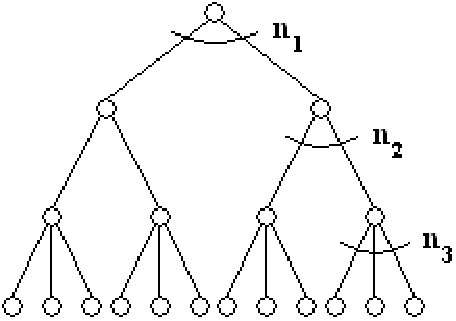
\includegraphics[bb = -40 0 0 160, scale=0.7]{counting}

It has branching factor $n_1$ at the root, $n_2$ at every node at the second level,...,
$n_k$ at every node at the $k$-th level. Each node at level $k+1$ (a leaf node)
represents one possible way of making the object by making a succession of $k$ choices. 
So the number of distinct objects that can be made is equal to the number of leaves in the 
tree. Moreover, the number of leaves in the tree is the product $n_1 \cdot n_2 \cdot n_3 \cdots n_k$.
For example, if $n_1 = 2$, $n_2 = 2$, and $n_3 = 3$, then there
are 12 leaves (i.e., outcomes). 

\section*{Counting Sets}
Consider a slightly different question. We would like to pick $k$
distinct elements of $S = \{1,2,\cdots,n\}$ (i.e. without repetition), but
we do not care about the order in which we picked the $k$ elements. For example, picking elements $1,\dots,k$
is considered the same outcome as picking elements $2,\dots,k$ and picking $1$ as the
last ($k^{th}$ element). Now how many ways are there to choose these elements? 

When dealing a hand of cards, say a poker hand, it is often more 
natural to count the number of distinct hands (i.e., the set 
of $5$ cards dealt in the hand), rather than the order in 
which they were dealt. As we've seen
in the section above, if we are considering order, there are $52\cdot 51\cdot 50\cdot 49 \cdot 48 = \frac{52!}{47!}$
outcomes. But how many distinct hands of $5$ cards are there? Here is another way of asking the question:
each such $5$ card hand is just a subset of $S$ of cardinality $5$. So we are asking how many $5$ element
subsets of $S$ are there?

Here is a clever trick for counting the number of distinct subsets of $S$ with exactly $5$ elements.
Create a bin corresponding to each such $5$ element subset. Now 
take all the sequences of $5$ cards and distribute them into these bins in the natural way. 
Each sequence gets placed in the bin corresponding to the set of $5$ elements in the sequence. 
Thus if the sequence is $(2,1, 3, 5, 4)$, then it is placed in the bin labeled $\{1, 2, 3, 4, 5\}$. 
How many sequences are placed in each bin? The answer is exactly $5!$, since there are exactly
$5!$ different ways to order $5$ cards. 

Recall that our goal was to compute the number of $5$ element subsets, which now corresponds
to the number of bins. We know that there are $\frac{52!}{47!}$ 5-card sequences, and there are $5!$ sequences
placed in each bin. The total number of bins is therefore $\frac{52!}{47!5!}$. 

This quantity $\frac{n!}{(n-k)!k!}$ is used so often that there
is special notation for it: $n \choose k$, pronounced {\em n choose k}.
This is the number of ways of picking $k$ distinct elements from $S$,
where the order of placement does not matter. 
Equivalently, it's the number of ways of choosing $k$ objects
out of a total of~$n$ objects, where the order of the choices does
not matter.

The trick we used above is actually our second rule of counting: 

\noindent
{\bf Second Rule of Counting:}
Assume an object is made by a succession of choices, and the order
in which the choices is made does not matter. Let $A$ be the
set of ordered objects and let $B$ be the set of unordered objects.
If there exists a $k$ to 1 function $f$ from $A$ to $B$, 
we can count the number of ordered objects (pretending that the order matters)
and divide by $k$ (the number of ordered objects per unordered objects) to obtain $|B|$,
the number of unordered objects.

Note that we are assuming the number of ordered objects is the same for every 
unordered object; the rule cannot be applied otherwise.  Here is another way of 
picturing the second rule of counting:

\begin{center}
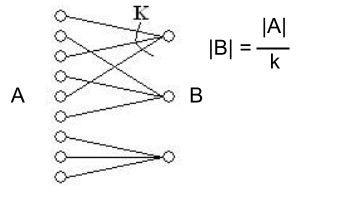
\includegraphics[scale=.6]{counting2.png}
\end{center}

The function $f$ simply places the ordered outcomes into bins corresponding to the unordered outcomes. 
In our poker hand example, $f$ will map $5!$ elements in the domain of the function (the set of ordered $5$ card outcomes)
to one element in the range (the set of $5$ element subsets of $S$). 
The number of elements in the range of the function is therefore $\frac{52!}{47!5!}$. 



\section*{Sampling with Replacement}

Sometimes we wish to consider a different scenario where we are still picking $k$ elements out of 
an $n$ element set $S = \{1,2,\cdots,n\}$ one at a time (order matters). The difference is that after we pick an element
for our sequence, we throw it back into $S$ so we can pick it again. 
How many such sequences of 
$k$ elements can we obtain? We can use the first rule of counting. Since we have $n$ choices
in each trial, $n_1 = n_2 = \ldots = n _k = n$. Then we have a grand total of $n^k$ sequences. 

This type of sampling is called {\it sampling with replacement}; 
multiple trials can have the same outcome.
Card dealing is a type of {\it sampling without replacement}, since two trials cannot both have
the same outcome (one card cannot be dealt twice). 

\subsection*{Coin Flipping}
Let us return to coin flipping. How many different outcomes are there if we flip a coin $k$ times? By outcome, 
we mean the string of results: i.e. 001 would represent
2 tails followed by a heads. We can picture this using the tree below, which depicts the possible outcomes when $k = 3$:

\begin{center}

\includegraphics[scale=.6]{coinflip.png}
\end{center}

Here $S = \{0,1\}$. This is a case of sampling with replacement; multiple coin flips could result in tails (we could pick 
the element 0 from set $S$ in multiple trials). Order also matters - strings $001$
and $010$ are considered different outcomes. By the reasoning above (using the first rule of counting) we have a total 
of $n^k = 2^k$ distinct outcomes, since $n = 2$. 

\subsection*{Rolling Dice}

Let's say we roll two dice, so $k = 2$ and $S = \{1,2,3,4,5,6\}$. How many possible outcomes are there? In this setting, ordering matters;
obtaining 1 with the first die and 2 with the second is different from obtaining 2 with the first and 1 with
the second. We are sampling with replacement, since we can obtain the same result on both dice. 

The setting is therefore the same as the coin flipping example above (order matters and we are sampling 
with replacement), so we can use the first rule of counting in the same manner. 
The number of distinct outcomes is therefore $n^2 = 6^2 = 36$.



\subsection*{Sampling with replacement, but where order does not matter}

Say you have unlimited quantities of apples,
bananas and oranges. You want to select 5 pieces of fruit to make a fruit salad.
How many ways are there to do this? In this example, $S = \{1,2,3\}$, where 1 represents 
apples, 2 represents bananas, and 3 represents oranges. $k = 5$ since we 
wish to select 5 pieces of fruit. Ordering does not matter; selecting an apple
followed by a banana will lead to the same salad as a banana followed by
an apple. 

This scenario is much more tricky to analyze. It is natural to apply the second rule of counting
because order does not matter. So we first pretend that order matters, and then the number of 
ordered objects is $3^5$ as discussed above. How many ordered options are there
for every unordered option? The problem is that this number differs depending on which
unordered object we are considering. Let's say the unordered object is an
outcome with 5 bananas. There is only one such ordered outcome. But if we are considering
4 bananas and 1 apple, there are 5 such ordered outcomes (represented as 12222,21222,22122,22212,22221). 

Now that we see the second rule of counting will not help, can we look at this problem
in a different way? Let us first generalize back to our original setting: we have a set $S = \{1,2,\cdots,n\}$ and we would like to know
how many ways there are to choose multisets (sets with repetition)
of size $k$.  Remarkably, we can model this problem in terms of binary strings.

Assume we have 1 bin for each element from set $S$, so $n$ bins. For example,
if we selected 2 apples and 1 banana, bin 1 would have 2 elements
and bin 2 would have 1 element.  In order to 
count the number of multisets, we need to count how many different ways there
are to fill these bins with $k$ elements. We don't care about the order of the bins themselves,
just how many of the $k$ elements each bin contains. Let's represent each of the $k$
elements by a 0 in the binary string, and separations between bins by a 1. Consider
the following picture: 

\begin{center}
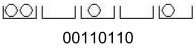
\includegraphics[scale=.8]{bin4.png}
\end{center}

This would be a sample placement where $S = \{1,\cdots,5\}$ and $k = 4$. 
Counting the number of multi sets
is now equivalent to counting the number of 
placements of the
$k$ 0's. 
We have just reduced what seemed like a very complex problem to
a question about a binary string, simply by looking at it from a different perspective!  

How many ways can we choose these locations? The length
of our binary string is $k + n - 1$, and we are choosing which $k$ locations
should contain 0's. The remaining $n-1$ locations will contain 1's.
Once we pick a location for one zero, we cannot pick it again; repetition
is not allowed. Picking location 1 followed by location 
2 is the same as picking location 2 followed by location 1, so ordering does not matter.
It follows that all we wish to compute is the number of ways of picking $k$ elements from $k + n - 1$ elements, without
replacement and where the order of placement does not matter. This is given by $n + k - 1\choose k$,
as discussed in the Counting Sets section above. This is therefore the number of ways
in which we can choose multisets of size $k$ from set $S$. 

Returning to our example above, the number of ways of picking 5 pieces of fruit is exactly ${3+5-1 \choose 5} = {7 \choose 5}$

Notice that we started with a problem which seemed very different from previous examples,
but, by viewing it from a certain perspective, we were able to use previous techniques (those used
in counting sets) to find a solution! This is key to many combinatorial arguments as we will
explore further in the next section. 


\section*{Combinatorial Proofs}

Combinatorial arguments are interesting because they rely on intuitive counting arguments
rather than algebraic manipulation. We can prove complex facts, such as 
${n \choose k+1} = {n-1 \choose k} + {n-2 \choose k} + \cdots + {k \choose k}$.
You can directly verify this identity by algebraic manipulation. But you can also do this 
by interpreting what each side means as a combinatorial process. The left hand side is just
the number of ways of choosing a $k+1$ element subset from a set of $n$ items. Let us think about a different
process that results in the choice of a $k+1$ element subset. We start by picking the lowest numbered
element in the subset. It is either the first element of the set or the second or the third or ... 
If we choose the first element, we must now choose $k$ elements out of the remaining $n-1$ 
which we can do in ${n-1 \choose k}$ ways. If instead the lowest numbered element we picked is 
the second element then we still have to choose $k$ elements from the remaining $n-2$ which can
be done in ${n-2 \choose k}$ ways. Moreover all these subsets are distinct from those where the 
lowest numbered element was the first one. So we should add the number of ways of choosing each 
to the grand total. Proceeding in this way, we split up the process into cases according
to the first (i.e., lowest-numbered) object we select, to obtain:
$$
\textbf{First element selected is either} \left\{ 
\begin{array}{cc}
\text{element 1},&$ ${n-1 \choose k} \vspace{.2cm}\\
\text{element 2},&$ ${n-2 \choose k} \vspace{.2cm}\\
\text{element 3},&$ ${n-3 \choose k} \vspace{.2cm}\\
\vdots\\
\text{element} (n-k),&$ ${k \choose k}
\end{array}\right.
$$
(Note that the lowest-numbered object we select cannot be higher than $n-k$ as we have to
select $k$ distinct objects.)

The last combinatorial proof we will do is the following: ${n \choose
0} + {n \choose 1} + \cdots + {n \choose n} = 2^n$. To see this,
imagine that we have a set $S$ with $n$ elements.  On the left hand
side, the $i^{th}$ term counts the number of ways of choosing a
subset of~$S$ of size exactly~$i$; so the sum on the left hand side
counts the total number of subsets (of any size) of~$S$.

We claim that the right hand side ($2^n$) does indeed also count the total
number of subsets.  To see this, just identify a subset with an $n$-bit
vector, where in each position~$j$ we put a~1 if the $j$th element is in
the subset, and a~0 otherwise.  So the number of subsets is equal to
the number of $n$-bit vectors, which is~$2^n$ (there are 2 options for
each bit).  Let us look at
an example, where $S = \{1,2,3\}$ (so $n=3$).  Enumerate all
$2^3 = 8$ possible subsets of $S$:
$\{\{\},\{1\},\{2\},\{3\},\{1,2\},\{1,3\},\{2,3\},\{1,2,3\}\}$. The
term ${3 \choose 0}$ counts the number of ways to choose a subset of
$S$ with 0 elements; there is only one such subset, namely the empty
set. There are ${3\choose 1}=3$ ways of choosing a subset with 1 element,
${3\choose 2}=3$ ways of choosing
a subset with 2 elements, and ${3\choose 3}=1$
way of choosing a subset with 3 elements (namely, the subset consisting
of the whole of~$S$).  Summing, we get $1+3+3+1 = 8$, as expected.
\end{document}

